\begin{frame}
   \frametitle{Planning over C-Space Families}
   \begin{tikzpicture}[font=\small]
   \tikzset{>=latex} % arrow heads
   \draw[step=1,black!15,very thin,opacity=\gridopacity] (0,0) grid (12,8);

   \node[fill=black!2,draw=black!5,rounded corners,minimum height=7.45cm,anchor=north] at (3.5,7.7)
   {\begin{minipage}{4.0cm}
      Structure of joint C-space \dots%
      \vspace{-0.25cm}%
      \begin{center}
         \includegraphics[width=3cm]{build/family-composite/plot-g-manifold}
      \end{center}%
      \vspace{-0.25cm}%
      \dots projected onto $\mathcal{C}_{\ms{robot}}$:%
      \vspace{-0.25cm}%
      \begin{center}
         \includegraphics[width=3cm]{build/multiple-sets}
      \end{center}
   \end{minipage}};

   \node[fill=blue!10,draw=blue!20,rounded corners,align=center,minimum width=5.0cm,minimum height=1.5cm,anchor=north] at (8.5,7.7)
   {$\arraycolsep=1.5pt \begin{array}{cl}
      x(\xi)\!: & \mbox{execution cost} \;(\mathcal{C}_{\ms{free}}) \\
      \hat{x}(\xi)\!: & \mbox{execution cost estimate} \\
      \grave{p}(\xi)\!: & \mbox{planning cost estimate}
   \end{array}$};

   \node[fill=black!2,draw=black!5,rounded corners,minimum width=5.0cm,minimum height=5.75cm,anchor=north] at (8.5,6.0)
   {\begin{minipage}{4.5cm}
      Assign to each roadmap edge $\xi_e$
      a belief state $b_e$
      which captures belief over subset membership:%
      \vspace{-0.2cm}%
      \begin{center}
         \includegraphics[width=3cm]{build/family-belief-graph-example-wrels-policy}
      \end{center}%
      \vspace{-0.2cm}%
      A shortest path from $b_e$ of belief transitions
      yields $\grave{p}(\xi)$.
   \end{minipage}};

   \end{tikzpicture}
\end{frame}


%\begin{frame}
%   \frametitle{Talk Outline}
%   \begin{tikzpicture}[font=\small]
%      \tikzset{>=latex} % arrow heads
%      \draw[step=1,black!15,very thin,opacity=\gridopacity] (0,0) grid (12,8);
%
%      \node[fill=blue!15,minimum width=11cm] at (6,7.5) {\strut How to Optimize?};
%
%      \node[fill=black!3,minimum width=5cm,minimum height=3cm] (lazysp) at (3.25,5.6) {};
%      \node[anchor=north] at (lazysp.north) {\strut Lazy Pathfinding};
%      \node[draw=black!30,fill=white,inner sep=5pt] at (3.25,5.4) {
%         \includegraphics[width=3.8cm]{build/lazysp-icon}};
%
%      \node[fill=black!3,minimum width=5cm,minimum height=3cm] (ibid) at (8.75,5.6) {};
%      \node[anchor=north] at (ibid.north) {\strut Dynamic Pathfinding};
%      \node[draw=black!30,inner sep=0pt] at (8.75,5.4) {
%         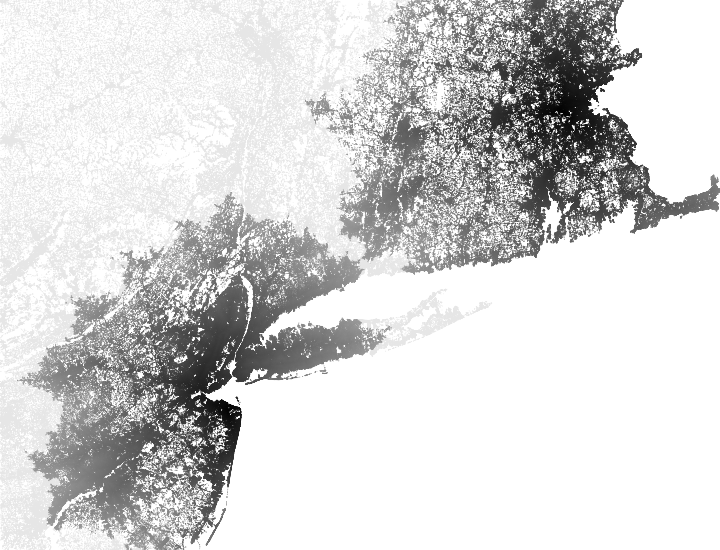
\includegraphics[width=2.9cm]{figs/incbi-road-ne/singleshot/example-bidijkstra.png}};
%
%      \node[fill=blue!15,minimum width=11cm] at (6,3.5) {\strut What to Optimize?};
%
%      \node[fill=black!3,minimum width=5cm,minimum height=3cm] (utility) at (3.25,1.6) {};
%      \node[anchor=north] at (utility.north) {\strut Maximizing Utility};
%      \node at (3.25,1.35) {\includegraphics[width=2.5cm]{build/pvx-utility-anytime}};
%
%      \node[fill=black!3,minimum width=5cm,minimum height=3cm] (family) at (8.75,1.6) {};
%      \node[anchor=north] at (family.north) {\strut Utility in C-Space Familes};
%      \node at (8.75,1.4) {\includegraphics[width=3.0cm]{build/multiple-sets}};
%
%      \only<2>
%      {
%      }
%      
%   \end{tikzpicture}
%\end{frame}

%\begin{frame}
%   \frametitle{Planning over C-Space Families}
%   
%\end{frame}

%\begin{frame}
%   \frametitle{Maximizing Utility: HERB Bin Experiments}
%   \begin{tikzpicture}[font=\small]
%      \tikzset{>=latex} % arrow heads
%      \draw[step=1,black!15,very thin,opacity=\gridopacity] (0,0) grid (12,8);
%
%      \node at ( 6,6.5) {
%         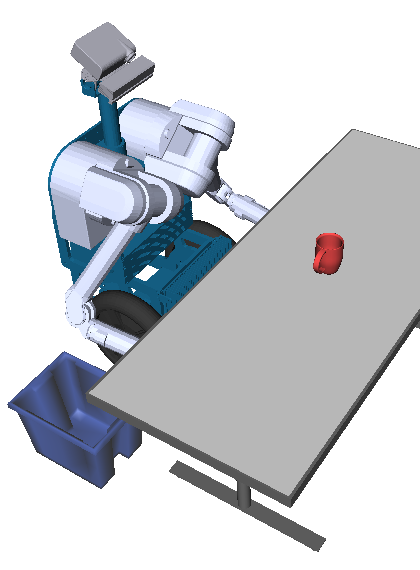
\includegraphics[width=1.7cm]{figs/herbbin/step0cropped.png}
%         \;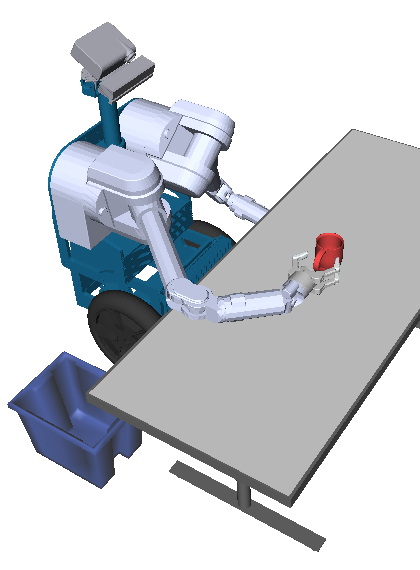
\includegraphics[width=1.7cm]{figs/herbbin/step01cropped.png}};
%
%      \node at ( 6,2.5) {\includegraphics[width=9cm]{build/multistep-prescribed/herbbinnom-g1ll}};
%      
%   \end{tikzpicture}
%\end{frame}

%\begin{frame}
%   \frametitle{Maximizing Utility: Workcell Experiments}
%   \begin{tikzpicture}[font=\small]
%      \tikzset{>=latex} % arrow heads
%      \draw[step=1,black!15,very thin,opacity=\gridopacity] (0,0) grid (12,8);
%
%      %\node at ( 6,6.5) {
%      %   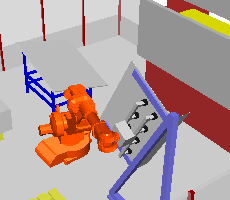
\includegraphics[width=2.7cm]{figs/workcell/cropped-config-f.png}
%      %   \;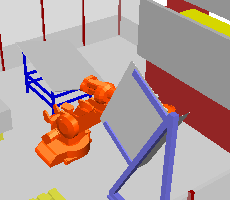
\includegraphics[width=2.7cm]{figs/workcell/cropped-config-g.png}};
%
%      \node[inner sep=0pt] (vidnode) at (6,6.5) {%
%         \href{\tikzvidtarget{incbi-roadne}}{%
%         \includegraphics[width=4cm]{videos/workcell-cropped.png}}};
%      \tikzvidplayat{incbi-roadne}{vidnode}{videos/workcell-cropped.mp4}{}
%
%      \node at ( 6,2.5) {\includegraphics[height=4cm]{build/multistep-prescribed/workcell-g1ll-lemuronly}};
%      
%   \end{tikzpicture}
%\end{frame}

\begin{frame}
   \frametitle{Maximizing Utility over C-Space Families}
   \begin{tikzpicture}[font=\small]
      \tikzset{>=latex} % arrow heads
      \draw[step=1,black!15,very thin,opacity=\gridopacity] (0,0) grid (12,8);

      %\node[draw=black!40,rounded corners,inner sep=2pt,anchor=north] at ( 3.75,6.4) {
      %   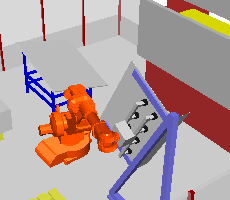
\includegraphics[width=2.7cm]{figs/workcell/cropped-config-f.png}
      %   \;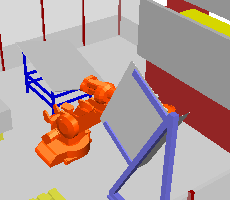
\includegraphics[width=2.7cm]{figs/workcell/cropped-config-g.png}};

      \node[inner sep=0pt] (herbbin-cropped) at (3.5,6.0) {%
         \href{\tikzvidtarget{herbbin-cropped}}{%
         \includegraphics[width=3.5cm]{videos/herbbin-cropped.png}}};
      \tikzvidplayat{herbbin-cropped}{herbbin-cropped}{videos/herbbin-cropped.mp4}{-loop 0}

      \node[inner sep=0pt] (workcell-cropped) at (8.5,6.0) {%
         \href{\tikzvidtarget{workcell-cropped}}{%
         \includegraphics[width=4cm]{videos/workcell-cropped.png}}};
      \tikzvidplayat{workcell-cropped}{workcell-cropped}{videos/workcell-cropped.mp4}{-loop 0}

      \tikzvidtargetboth{both-cropped}{herbbin-cropped}{workcell-cropped}

      \node at (3.2,2.2) {\includegraphics[height=4cm]{build/multistep-prescribed/herbbinnom-g1ll-lemuronly}};

      \node at (8.2,2.2) {\includegraphics[height=4cm]{build/multistep-prescribed/workcell-g1ll-lemuronly}};
      
   \end{tikzpicture}%
   \begin{tikzpicture}[remember picture,overlay]
      \node[anchor=south west,fill=black!10,inner sep=0pt] at (current page.south west)
      {\href{\tikzvidtarget{both-cropped}}{\tikz{\node[minimum width=2cm,minimum height=0.3cm]{}}}};
   \end{tikzpicture}%
\end{frame}
